%% ============================================================
%%  INFORME DE PROYECTO - TÉCNICAS DE CONTROL
%%  Sistema: Aeropéndulo
%%  Universidad Nacional de Colombia - Sede Bogotá
%%  Compilar con: pdflatex
%% ============================================================
\documentclass[11pt,letterpaper]{article}

% ---------- Codificacion e idioma ----------
\usepackage[utf8]{inputenc}
\usepackage[T1]{fontenc}
\usepackage[spanish,es-noshorthands,es-tabla]{babel}
\usepackage{lmodern}
\usepackage{microtype}

% ---------- Pagina y margenes ----------
\usepackage[top=2.5cm,bottom=2.3cm,left=2.3cm,right=2.3cm,headheight=28pt]{geometry}
\usepackage{fancyhdr}
\usepackage{lastpage}
\usepackage{setspace}
\setstretch{1.12}

% ---------- Matematicas ----------
\usepackage{amsmath,amssymb,mathtools}
\usepackage{siunitx}
\sisetup{output-decimal-marker={,}}

% ---------- Graficos y tablas ----------
\usepackage{graphicx}
\usepackage{xcolor}
\usepackage{booktabs}
\usepackage{array}
\usepackage{multirow}
\usepackage{tabularx}
\usepackage{float}
\usepackage[font=small,labelfont=bf]{caption}
\usepackage{subcaption}
\usepackage{tcolorbox}
\tcbuselibrary{skins,breakable}
\graphicspath{{Imagenes/}{./}}

% ---------- Diagramas con TikZ ----------
\usepackage{tikz}
\usetikzlibrary{shapes.geometric,arrows.meta,positioning,calc}

% ---------- Codigo MATLAB / C++ ----------
\usepackage{listings}

\definecolor{mlkeyword}{RGB}{0,0,255}
\definecolor{mlcomment}{RGB}{0,128,0}
\definecolor{mlstring}{RGB}{160,32,240}
\definecolor{mlbg}{RGB}{248,248,248}

\lstdefinestyle{matlabstyle}{
  language=Matlab,
  basicstyle=\ttfamily\footnotesize,
  keywordstyle=\color{mlkeyword}\bfseries,
  commentstyle=\color{mlcomment}\itshape,
  stringstyle=\color{mlstring},
  numbers=left,
  numberstyle=\tiny\color{gray},
  numbersep=8pt,
  backgroundcolor=\color{mlbg},
  frame=single,
  rulecolor=\color{black!25},
  breaklines=true,
  breakatwhitespace=false,
  tabsize=4,
  showstringspaces=false,
  columns=fullflexible,
  keepspaces=true,
  xleftmargin=14pt,
  captionpos=b,
  literate=
    {a}{{\'{a}}}1 {e}{{\'{e}}}1 {i}{{\'{i}}}1 {o}{{\'{o}}}1 {u}{{\'{u}}}1
    {A}{{\'{A}}}1 {E}{{\'{E}}}1 {I}{{\'{I}}}1 {O}{{\'{O}}}1 {U}{{\'{U}}}1
    {n}{{\~{n}}}1 {N}{{\~{N}}}1
}

\lstset{style=matlabstyle}
\renewcommand{\lstlistingname}{C\'{o}digo}

% ---------- Listas y enlaces ----------
\usepackage{enumitem}
\setlist[enumerate,1]{label=\textbf{\arabic*.},leftmargin=*}
\setlist[enumerate,2]{label=\textbf{\alph*)},leftmargin=1.8em}
\usepackage[hidelinks]{hyperref}

% ============================================================
%  DATOS DEL TRABAJO
% ============================================================
\newcommand{\universidad}{Universidad Nacional de Colombia}
\newcommand{\facultad}{Facultad de Ingeniería}
\newcommand{\departamento}{Departamento de Ingeniería Mecánica y Mecatrónica}
\newcommand{\programa}{Ingeniería Mecatrónica}
\newcommand{\curso}{Técnicas de Control}
\newcommand{\tipo}{Informe de Proyecto}
\newcommand{\profesor}{Prof.\ Jorge Iván Sofrony Esmeral}
\newcommand{\periodo}{2026-II}
\newcommand{\fecha}{\today}

\newcommand{\nombregrupo}{Modelado, Caracterización Experimental y Control de un Aeropéndulo}

% Integrantes
\newcommand{\integranteA}{Samuel David Negrete Lancheros}
\newcommand{\integranteB}{Jes\'us David Sánchez Cobos}
\newcommand{\integranteC}{Leonardo Acevedo Monroy}
\newcommand{\integranteD}{Ariel Giovanni Cárdenas Santisteban}

% Correos institucionales
\newcommand{\correoA}{\textit{snegrete@unal.edu.co}}
\newcommand{\correoB}{\textit{jdsanchezco@unal.edu.co}}
\newcommand{\correoC}{\textit{leacevedo@unal.edu.co}}
\newcommand{\correoD}{\textit{arcardenass@unal.edu.co}}

% ============================================================
%  ENCABEZADO Y PIE
% ============================================================
\pagestyle{fancy}
\fancyhf{}
\lhead{\small\textbf{\curso}}
\chead{\small\tipo}
\rhead{\small\periodo}
\lfoot{\small\departamento{} -- \programa}
\rfoot{\small Página~\thepage\ de~\pageref{LastPage}}
\renewcommand{\headrulewidth}{0.4pt}
\renewcommand{\footrulewidth}{0.4pt}

% ============================================================
%  MACROS
% ============================================================
\newcommand{\dd}{\,\mathrm{d}}
\DeclarePairedDelimiter{\abs}{\lvert}{\rvert}
\DeclarePairedDelimiter{\norm}{\lVert}{\rVert}

\numberwithin{equation}{section}
\setlength{\parindent}{0pt}
\setlength{\parskip}{0.6em}

% ============================================================
\begin{document}

% ---------- Portada ----------
\begin{center}
  {\large\bfseries \universidad}\\[2pt]
  {\normalsize \facultad}\\[1pt]
  {\normalsize \departamento}\\[1pt]
  {\normalsize \programa}\\[10pt]
  {
\includegraphics[width=0.18\linewidth]{LogoUnalpng.png}}\\[8pt]
  {\Large\bfseries \curso}\\[2pt]
  {\large \tipo}\\[14pt]
  \begin{tcolorbox}[enhanced, colback=black!4, colframe=black!60,
      boxrule=0.6pt, arc=3pt, width=\linewidth, halign=center]
    {\LARGE\bfseries \nombregrupo}
  \end{tcolorbox}
\end{center}

\vspace{0.2cm}

% ---------- Integrantes ----------
\begin{center}
\renewcommand{\arraystretch}{1.4}
\begin{tabularx}{\linewidth}{
    >{\centering\arraybackslash}X
    >{\centering\arraybackslash}X
    >{\centering\arraybackslash}X
    >{\centering\arraybackslash}X}
  \toprule
  \textbf{\integranteA} &
  \textbf{\integranteB} &
  \textbf{\integranteC} &
  \textbf{\integranteD} \\[2pt]
  \correoA & \correoB & \correoC & \correoD \\
  \bottomrule
\end{tabularx}
\end{center}

\begin{center}
  \small \profesor \quad$\bullet$\quad \periodo \quad$\bullet$\quad \fecha
\end{center}

\vspace{0.1cm}
\hrule
\vspace{0.3cm}

% ---------- Resumen ----------
\begin{abstract}
\noindent Este informe presenta la estructura de diseño, caracterización experimental y modelado dinámico de un sistema tipo \textbf{aeropéndulo}. El prototipo físico está construido mediante corte láser en acrílico transparente y piezas en impresión 3D, incorporando un rodamiento de bolas en el pivote, actuación con motor DC y hélice, y sensado digital síncrono sobre bus $\mathrm{I^2C}$ (encoder magnético AS5600 e IMU BMI160) gestionado por un microcontrolador ESP32. Se establece el modelo dinámico rotacional de la planta, los protocolos experimentales para la determinación de la ganancia estática de empuje ($K_{uf}$) y el amortiguamiento viscoso ($B$), el cálculo de incertidumbres metrológicas y la linealización alrededor de puntos de operación para la posterior síntesis del sistema de control.
\\[4pt]
\textbf{Palabras clave:} Aeropéndulo, linealización alrededor de punto de operación, caracterización experimental, identificación paramétrica, control de posición.
\end{abstract}

% ============================================================
%  SECCIONES MODULARES
% ============================================================
% ============================================================
%  SECCIÓN 1: INTRODUCCIÓN
% ============================================================
\section{Introducción}

El aeropéndulo es una de las plataformas experimentales más interesantes en el ámbito de la teoría de control, debido a que el sistema exhibe un comportamiento dinámico no lineal y su susceptibilidad ante perturbaciones externas y dinámicas no modeladas.

\begin{figure}[ht]
    \centering
    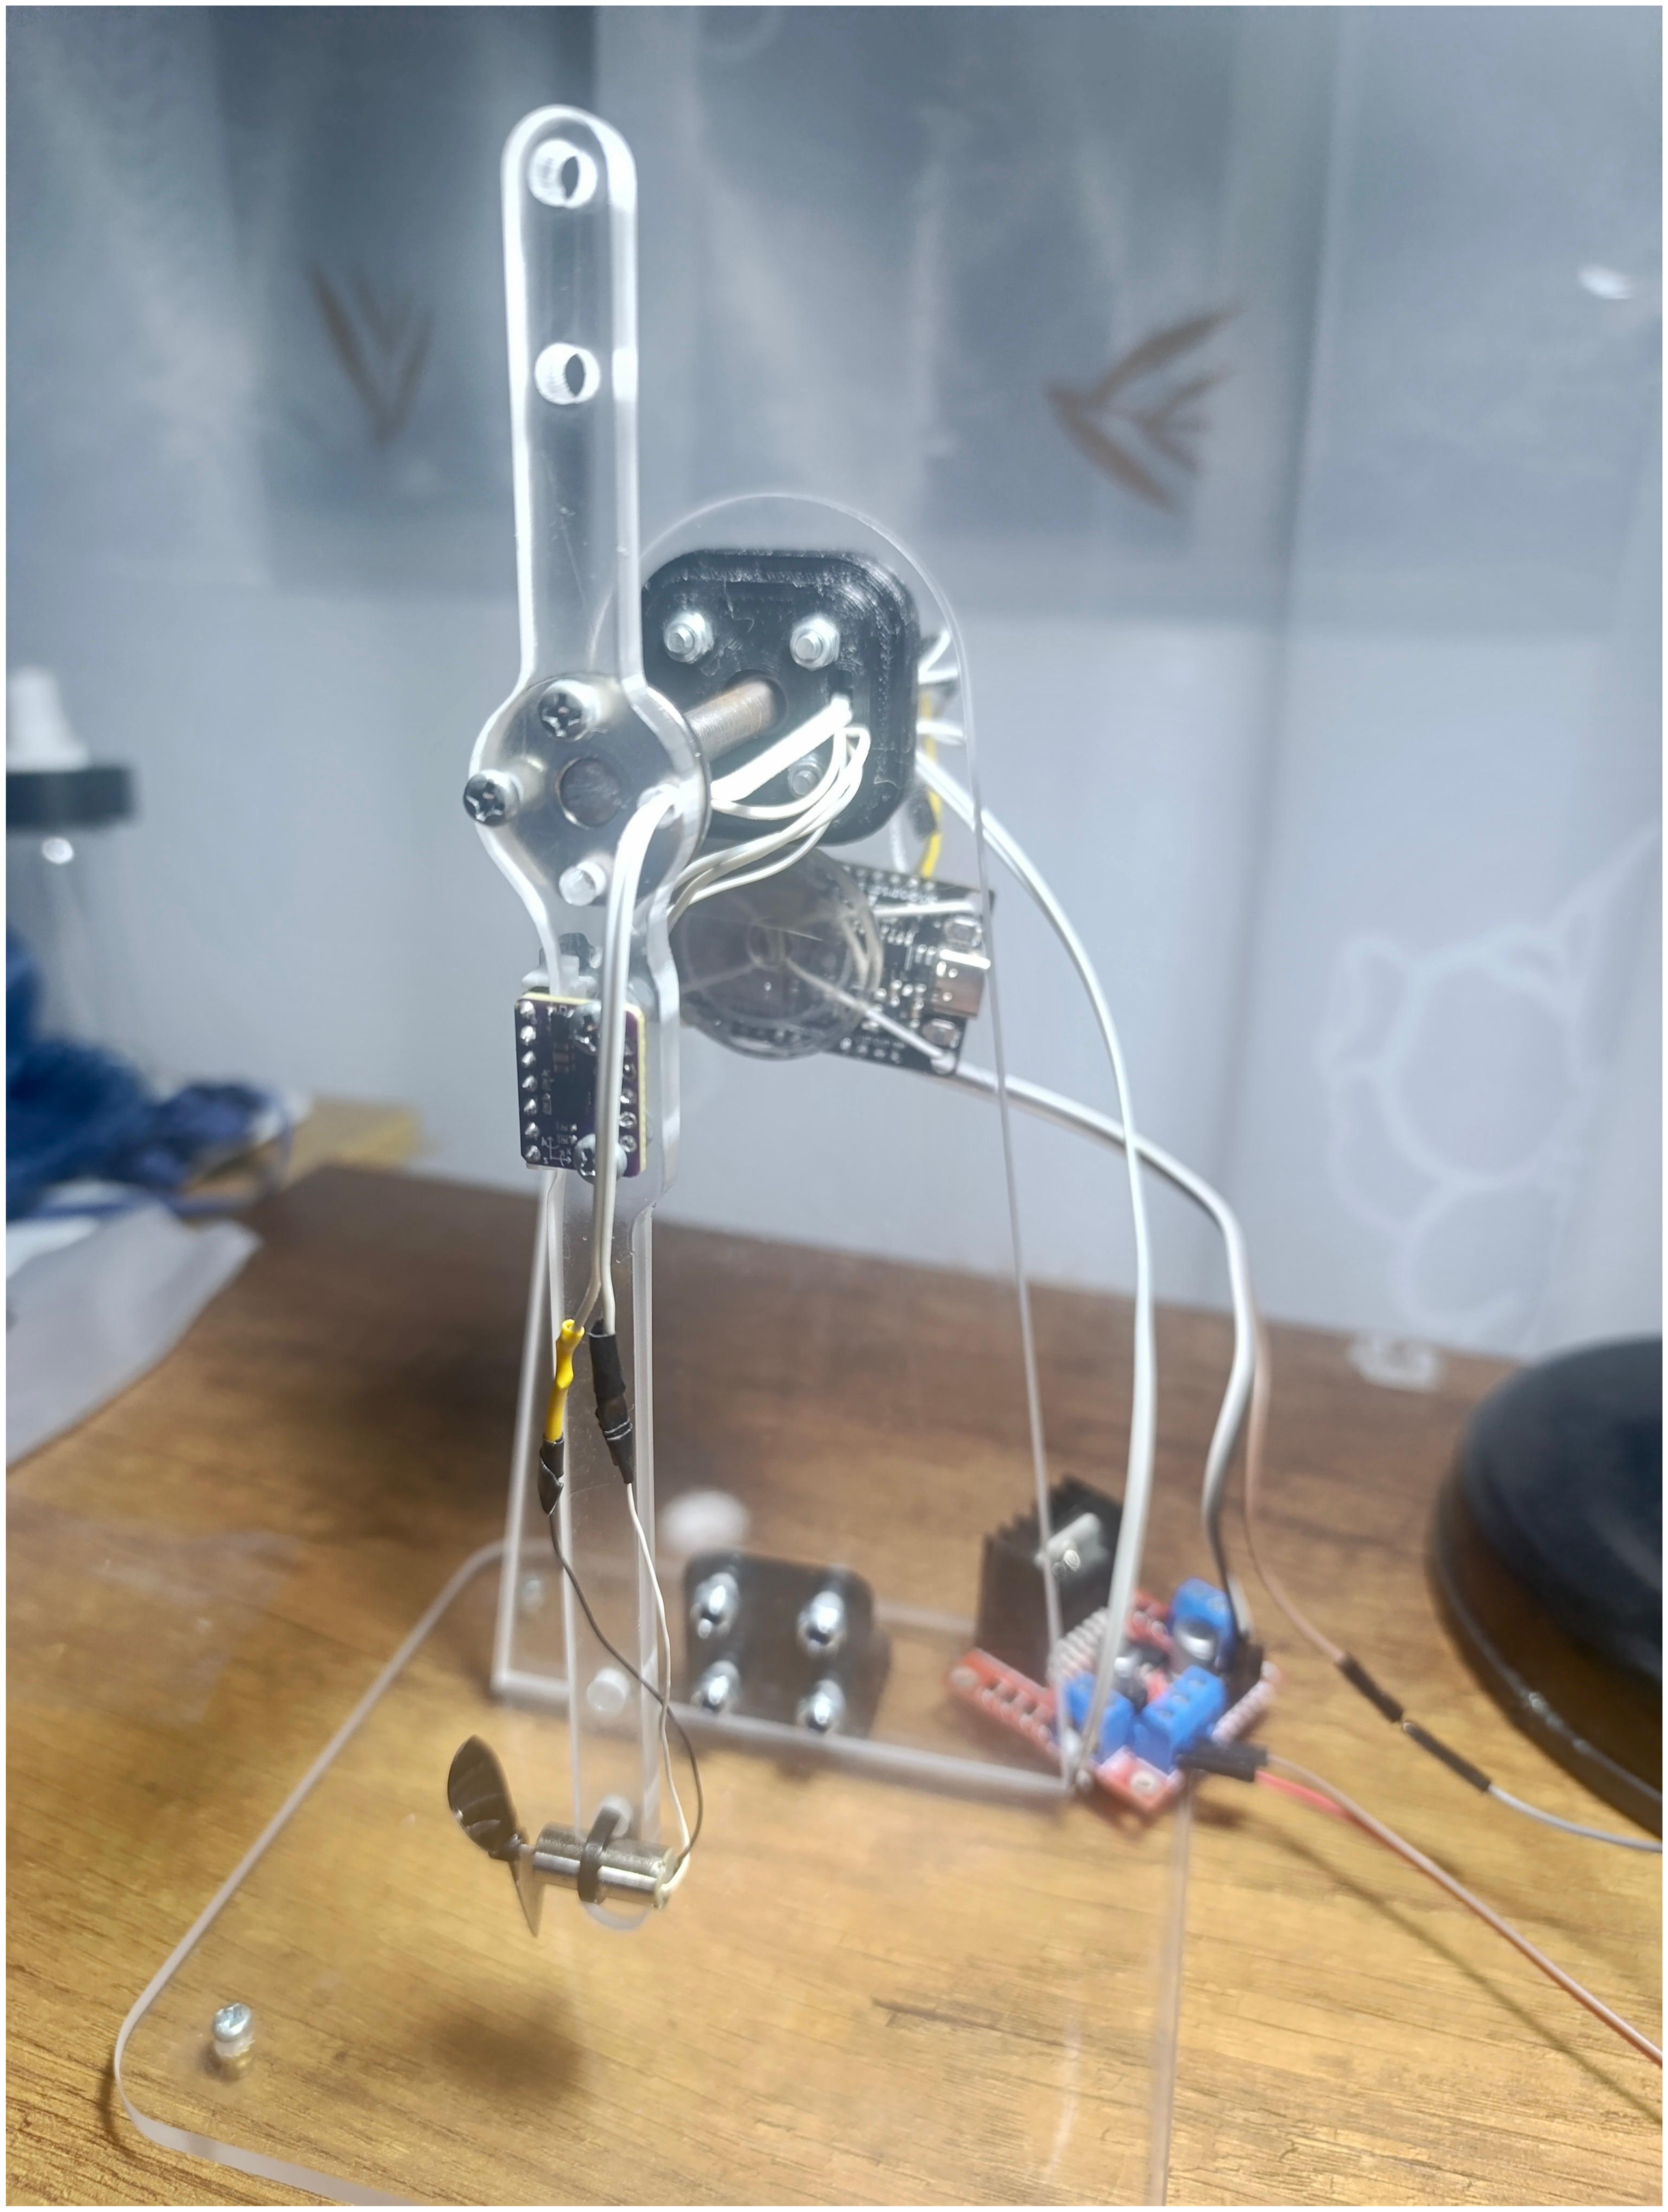
\includegraphics[width=0.3\textwidth]{Informe/Imagenes/planta.eps}
    \caption{Montaje del aeropéndulo}
    \label{fig:planta}
\end{figure}

El objetivo general de este proyecto es abordar el ciclo completo de ingeniería de control sobre un prototipo diseñado por nosotros mismo:
\begin{itemize}
  \item \textbf{Diseño e Integración Electromecánica:} Uso de procesos de manufactura rápida (corte láser e impresión 3D), un eje soportado por rodamientos y sensores controlados por un microcontrolador ESP32.
  
  \item \textbf{Caracterización Experimental de Parámetros:} Estimación de la ganancia del actuador ($K_{uf}$) y el coeficiente de fricción viscosa ($B$).
\end{itemize}

% ============================================================
%  SECCIÓN 2: PLANTEAMIENTO DEL PROBLEMA
% ============================================================
\section{Planteamiento del problema} 

\subsection{Definición del Sistema Físico y Arquitectura General}
El problema de control planteado consiste en gobernar la posición angular $\theta(t)$ de un aeropéndulo en el plano vertical mediante la generación de empuje por medio de un conjunto motor-hélice. La planta exhibe una dinámica no lineal debido al momento cuasado por la fuerza gravitacional dependiente de la posición angular y al comportamiento aerodinámico del flujo generado por las aspas.

La plataforma física comprende una serie de subsistemas interconectados:

\begin{enumerate}[leftmargin=*]
  \item \textbf{Unidad de Cómputo y Control (ESP32):} 
  Microcontrolador de 32 bits a $240\,\mathrm{MHz}$. Genera la señal de modulación por ancho de pulso (\textit{PWM}) para el control de potencia, gestiona la adquisición síncrona de datos por bus digital $\mathrm{I^2C}$ a $400\,\mathrm{kHz}$ (GPIO 21 para SDA y GPIO 22 para SCL) y ejecuta el lazo de control.

  \item \textbf{Etapa de Potencia y Actuador:} 
  Módulo driver / puente H conectado a los pines de control del ESP32 (GPIO 25 y 26). Excita un micromotor DC con hélice bipala de tracción, convirtiendo el ciclo de trabajo de PWM en una fuerza de empuje aerodinámico $F(t)$ aplicada en el extremo libre del brazo.

  \item \textbf{Estructura Mecánica y Montaje de Pivote:} 
  \begin{itemize}[noitemsep]
    \item \textbf{Chasis y brazo en acrílico:} Fabricados mediante corte por láser (\texttt{LaserFinal.dxf}). Comprende la base horizontal de soporte, la torre vertical de fijación y el brazo oscilante alargado.
    \item \textbf{Piezas en impresión 3D (PLA):} Fabricadas por manufactura aditiva FDM, incluyendo la brida soporte del pivote atornillada a la torre (\texttt{InsertoRoda.stl}), el soporte angular para el actuador (\texttt{Angulo.stl}) y los topes mecánicos.
    \item \textbf{Inserto con rodamiento y eje de acero:} El alojamiento impreso contiene un rodamiento de bolas sobre el eje cilíndrico de acero, minimizando la fricción por rozamiento directo.
  \end{itemize}

  \item \textbf{Subsistema Sensorial Digital:} 
  \begin{itemize}[noitemsep]
    \item \textbf{Encoder magnético absoluto AS5600:} Resolución de 12 bits ($4096$ pasos por revolución, resolución nominal de $0{,}0879^\circ$), comunicado a través del protocolo digital $\mathrm{I^2C}$. Montado en la parte posterior del pivote, enfrentado coaxialmente a un imán diametral fijado mediante un portaimán impreso (\texttt{TaponIman.stl}).
    \item \textbf{Unidad de Medición Inercial BMI160:} Sensor inercial montado directamente sobre el cuerpo del brazo de acrílico y conectado al bus $\mathrm{I^2C}$ (dirección $0\mathrm{x}68$), para el registro directo de la velocidad angular ($\dot{\theta} \equiv \mathrm{GyroZ}$).
  \end{itemize}
\end{enumerate}

\subsection{Esquema Funcional de Lazo Cerrado}
En la Figura~\ref{fig:esquema_lazo_cerrado} se representa el diagrama de bloques del sistema en lazo cerrado, detallando las señales que fluyen entre cada subsistema.

\begin{figure}[H]
  \centering
  \resizebox{\linewidth}{!}{%
  \begin{tikzpicture}[
      block/.style={draw, fill=blue!5, rounded corners=2pt, minimum height=1.0cm, minimum width=1.9cm, align=center, font=\small},
      sum/.style={draw, circle, inner sep=0pt, minimum size=6mm, font=\small},
      sensor/.style={draw, fill=green!6, rounded corners=2pt, minimum height=0.9cm, minimum width=2.2cm, align=center, font=\small},
      arrow/.style={-{Latex[scale=0.9]}, semithick},
      node distance=1.0cm and 0.8cm
    ]

    % Nodos directos
    \node (ref) {$\theta_{\mathrm{ref}}$};
    \node [sum, right=0.6cm of ref] (sum) {$+$};
    \node [block, right=0.7cm of sum] (ctrl) {\textbf{ESP32}\\\footnotesize Algoritmo};
    \node [block, right=0.9cm of ctrl] (driver) {\textbf{Driver}\\\footnotesize Puente H};
    \node [block, right=0.9cm of driver] (motor) {\textbf{Motor-Hélice}\\\footnotesize Empuje $K_{uf}$};
    \node [block, right=0.9cm of motor] (planta) {\textbf{Aeropéndulo}\\\footnotesize Dinámica rotacional};
    \node [right=0.8cm of planta] (salida) {$\theta(t)$};

    % Conexiones trayectoria directa
    \draw [arrow] (ref) -- node[above, font=\footnotesize] {$+$} (sum);
    \draw [arrow] (sum) -- node[above, font=\footnotesize] {$e(t)$} (ctrl);
    \draw [arrow] (ctrl) -- node[above, font=\footnotesize] {PWM} (driver);
    \draw [arrow] (driver) -- node[above, font=\footnotesize] {$V_{\mathrm{mot}}$} (motor);
    \draw [arrow] (motor) -- node[above, font=\footnotesize] {$F(t)$} (planta);
    \draw [arrow] (planta) -- (salida);

    % Lazo de realimentacion
    \node [sensor, below=1.2cm of $(driver)!0.5!(motor)$] (sensores) {\textbf{Sensores Digitales} $\mathbf{(I^2C)}$\\\footnotesize AS5600 ($\theta$) / BMI160 ($\dot{\theta}$)};

    \draw [arrow] ($(planta.east)+(0.3,0)$) |- (sensores.east);
    \draw [arrow] (sensores.west) -| node[pos=0.9, left, font=\footnotesize] {$-$} (sum);

  \end{tikzpicture}%
  }
  \caption{Esquema en bloques del aeropéndulo en lazo cerrado.}
  \label{fig:esquema_lazo_cerrado}
\end{figure}

\subsection{Señales de Entrada y Salida por Subsistema}
La Tabla~\ref{tab:senales_subsistemas} sintetiza las variables físicas y unidades que intervienen en cada etapa del sistema.

\begin{table}[H]
  \centering
  \caption{Mapeo de señales y unidades por subsistema.}
  \label{tab:senales_subsistemas}
  \renewcommand{\arraystretch}{1.25}
  \small
  \begin{tabularx}{\linewidth}{lXcc}
    \toprule
    \textbf{Subsistema} & \textbf{Descripción} & \textbf{Entrada} & \textbf{Salida} \\
    \midrule
    ESP32 / Algoritmo & Cálculo del control & Error $e(t)$ [rad] & Ciclo de trabajo [\%] \\
    Puente H + Motor  & Modulación $\to$ Empuje & PWM [\%] & Fuerza $F$ [N] \\
    Planta            & Torque $\to$ Giro angular & $F$ [N] & Posición $\theta$ [rad] \\
    Sensor AS5600     & Campo magnético $\to$ ángulo & Flujo magnético & Registro 12 bits \\
    Sensor BMI160     & Giroscopio & Giro físico & Velocidad $\dot{\theta}$ [$\mathrm{^\circ/s}$] \\
    \bottomrule
  \end{tabularx}
\end{table}
% ============================================================
%  SECCIÓN 3: ENTENDIMIENTO DE LA PLANTA Y MODELADO MATEMÁTICO
% ============================================================
\section{Entendimiento de la planta y Modelado Matem\'atico}

\subsection{Ecuaci\'on Diferencial No Lineal}
A partir del diagrama de cuerpo libre del aerop\'endulo en rotaci\'on plana alrededor del eje fijo del rodamiento, la sumatoria de momentos satisface:
\begin{equation}
  \sum \tau_O = I \ddot{\theta}(t)
\end{equation}

Considerando el torque generado por el empuje aerodin\'amico del motor $F(t) = K_{uf} u(t)$ a distancia radial $r$, el momento restaurador gravitacional con centro de masa a distancia $c$ y el amortiguamiento viscoso equivalente $B r^2$:
\begin{equation}
  I \ddot{\theta}(t) = r F(t) - B r^2 \dot{\theta}(t) - m g c \cos(\theta(t))
  \label{eq:dinamica_nolineal}
\end{equation}
donde $\theta(t)$ representa la posici\'on angular, $I$ el momento de inercia respecto al pivote, $m$ la masa oscilante, $g$ la aceleraci\'on de la gravedad y $u(t)$ la se\~nal de mando.

\subsection{Puntos de Equilibrio Estacionario}
En r\'egimen permanente estacionario ($\ddot{\theta}^* = 0$, $\dot{\theta}^* = 0$), la fuerza requerida para sostener un \'angulo de operaci\'on $\theta^*$ satisface:
\begin{equation}
  F^* = \frac{m g c}{r} \cos(\theta^*)
\end{equation}

\subsection{Linealizaci\'on Alrededor del Punto de Operaci\'on}
Dado el comportamiento fuertemente no lineal del t\'ermino trigonom\'etrico, se plantea una linealizaci\'on mediante aproximaci\'on por serie de Taylor alrededor de la condici\'on de operaci\'on $(\theta^*, \dot{\theta}^* = 0, F^*)$.

Definiendo las variables de desviaci\'on incremental:
\begin{equation}
  \Delta \theta(t) = \theta(t) - \theta^*, \qquad \Delta F(t) = F(t) - F^*
\end{equation}
la din\'amica linealizada resultante adquiere la forma:
\begin{equation}
  I \Delta \ddot{\theta}(t) + B r^2 \Delta \dot{\theta}(t) - m g c \sin(\theta^*) \Delta \theta(t) = r \Delta F(t)
  \label{eq:dinamica_linealizada}
\end{equation}

\subsection{Representaci\'on del Modelo (a definir con el equipo)}
A partir de la ecuaci\'on linealizada (\ref{eq:dinamica_linealizada}), se estructuran las v\'{\i}as de representaci\'on para la s\'{\i}ntesis del controlador:
\begin{itemize}[leftmargin=*]
  \item \textbf{Funci\'on de transferencia incremental $G(s)$:}
  \begin{equation}
    G(s) = \frac{\Delta \Theta(s)}{\Delta F(s)} = \frac{\dfrac{r}{I}}{s^2 + \dfrac{B r^2}{I} s - \dfrac{m g c \sin(\theta^*)}{I}}
  \end{equation}
  \item \textbf{Representaci\'on en espacio de estados:}
  Formulaci\'on matricial $\Delta \dot{\mathbf{x}} = \mathbf{A} \Delta \mathbf{x} + \mathbf{B} \Delta u$ para t\'ecnicas de control multivariable o moderno.
\end{itemize}

% ============================================================
%  SECCIÓN 4: DEFINICIÓN DE LA PLANTA Y CARACTERIZACIÓN DE PARÁMETROS
% ============================================================
\section{Definición de la planta y Caracterización de Parámetros}

La precisión predictiva del modelo linealizado en espacio de estados y la robustez del controlador a diseñar dependen de una determinación rigurosa de los parámetros físicos de la planta. Esta sección expone la metodología de obtención de parámetros directos e indirectos, junto con la cuantificación formal de sus fuentes de incertidumbre.

\subsection{Metodología de Obtención de Parámetros}

\subsubsection{Parámetros de Medición Directa}
Corresponden a magnitudes geométricas y físicas evaluadas directamente sobre la estructura física mediante instrumentación metrológica:
\begin{itemize}[leftmargin=*]
  \item \textbf{Radio al eje del motor ($r$):} Distancia medida con calibrador pie de rey de precisión desde el centro geométrico del eje del pivote hasta la línea de aplicación del empuje del motor:
  \begin{equation}
    r = 0.1350\,\mathrm{m} \quad (135.0\,\mathrm{mm})
  \end{equation}
  \item \textbf{Masa total oscilante ($m$):} Masa del ensamble móvil completo (brazo de acrílico, motor DC, hélice, soporte angular 3D, tornillería e insertos) registrada en una balanza analítica digital de resolución $0.1\,\mathrm{g}$:
  \begin{equation}
    m = 0.0300\,\mathrm{kg} \quad (30.0\,\mathrm{g})
  \end{equation}
  \item \textbf{Aceleración gravitacional ($g$):} Valor de referencia local para la ciudad de Bogotá D.C. ($2600\,\mathrm{m.s.n.m.}$):
  \begin{equation}
    g = 9.81\,\mathrm{m/s^2}
  \end{equation}
\end{itemize}

\subsubsection{Parámetros Indirectos y Caracterización Experimental}
Aquellas propiedades que no admiten medición directa requirieron el diseño de protocolos experimentales dedicados y modelado por elementos finitos/CAD:

\begin{enumerate}[leftmargin=*]
  \item \textbf{Distancia al Centro de Masa ($c$):} 
  Distancia axial desde el pivote hasta el centro de gravedad del conjunto móvil. Se determinó integrando las geometrías con ayuda del entorno CAD \textit{Autodesk Fusion 360}.
  \begin{equation}
    c = 0.0407\,\mathrm{m} \quad (40.68\,\mathrm{mm})
  \end{equation}

  \item \textbf{Momento de Inercia respecto al Pivote ($I$):} 
  Calculado en Fusion 360
  \begin{equation}
    I = I_G + m c^2 \approx 7.942 \times 10^{-5}\,\mathrm{kg\cdot m^2}
  \end{equation}
  Este valor resulta plenamente consistente con la frecuencia natural observada en los ensayos oscilatorios libres ($\omega_n \approx 12.28\,\mathrm{rad/s}$).

  \item \textbf{Ganancia Estática de Empuje del Actuador ($K_{uf}$):} 
  Esta ganancia engloba la conversión integral de la señal PWM en tensión efectiva sobre el motor, el par motor generado y el empuje aerodinámico de las aspas de la hélice. Dado que su dinámica eléctrica es significativamente más rápida que la respuesta mecánica del brazo, se modela como una ganancia estática $F(t) = K_{uf}\cdot u_{\mathrm{PWM}}(t)$.
  
  Para su caracterización se ejecutó el firmware \texttt{Varriación\_PWM} en el ESP32, aplicando una secuencia escalonada decreciente desde $90\%$ hasta $10\%$ de PWM en pasos de $2\%$, manteniendo cada nivel durante $5.0\,\mathrm{s}$ para extinguir los transitorios. A través del script de MATLAB \texttt{Gráfica\_y\_Lectura\_puerto.m}, se tomaron los promedios estables de ángulo $\theta_{\mathrm{est}}$ para cada nivel de PWM, despejando la fuerza estática requerida para el equilibrio:
  \begin{equation}
    \sum \tau = r F - m g c \cos(\theta_{\mathrm{est}}) = 0 \implies F = \frac{m g c}{r} \cos(\theta_{\mathrm{est}})
  \end{equation}
  Mediante un ajuste por regresión lineal de mínimos cuadrados ordinarios entre el PWM aplicado y la fuerza de sustentación resultante se identificó:
  \begin{equation}
    K_{uf} \approx 1.90 \times 10^{-3}\,\mathrm{N/\%}
  \end{equation}

  \item \textbf{Coeficiente de Fricción Viscosa ($B$):} 
  Para desacoplar el efecto de la fuerza motriz y caracterizar las fuerzas disipativas del rodamiento y la resistencia aerodinámica pasiva, se implementó el método del \textbf{decremento logarítmico} sobre la oscilación libre subamortiguada (\texttt{Friccion} y \texttt{Envolvente.m}).
  
  El procedimiento consistió en:
  \begin{enumerate}[label=\alph*)]
    \item Posicionar el brazo en un ángulo inicial estacionario aplicando un ciclo de trabajo base de $75\%$.
    \item Interrumpir s\'ubita e instantáneamente la señal PWM a cero ($u = 0$), permitiendo que el aeropéndulo oscile libremente hacia su punto de equilibrio natural.
    \item Registrar la serie temporal del ángulo $\theta(t)$ y la velocidad $\dot{\theta}(t)$ mediante el encoder AS5600 y la IMU BMI160 a $115200\,\mathrm{baud}$.
    \item Identificar los instantes de tiempo $t_k$ y amplitudes de los máximos y mínimos locales $(\abs{\theta_k})$, ajustando una envolvente exponencial teórica:
    \begin{equation}
      \theta_{\mathrm{env}}(t) = A_0 e^{-\sigma t} \implies \ln \abs{\theta_k} = \ln(A_0) - \sigma t_k
    \end{equation}
    \item A partir de la pendiente de la recta semilogarítmica se determinó la tasa de decaimiento experimental $\sigma \approx 0.8176\,\mathrm{s^{-1}}$ y el periodo de oscilación amortiguada $T_d \approx 0.512\,\mathrm{s}$. Conforme a la ecuación característica de segundo orden:
    \begin{equation}
      2\zeta\omega_n = \frac{B r^2}{I} = 2\sigma \implies B = \frac{2\sigma I}{r^2} \approx 7.13 \times 10^{-3}\,\mathrm{N\cdot s/m}
    \end{equation}
  \end{enumerate}
\end{enumerate}


% ============================================================
%  SECCIÓN 5: DISEÑO DEL CONTROLADOR
% ============================================================
\section{Diseño del Controlador}

\subsection{Criterios y Especificaciones de Diseño}

\subsection{Propuesta de Estructura de Control}

\subsection{Implementación Computacional}

% ============================================================
%  SECCIÓN 6: RESULTADOS Y COMPARACIÓN
% ============================================================
\section{Resultados y Comparación}

\subsection{Validación de la Respuesta en Simulación}
% Contraste de la respuesta transitoria del modelo no lineal simulado en SimulinkPrueba.slx
% frente al modelo linealizado matricialmente.

\subsection{Respuesta Experimental en la Planta Física}



% ============================================================
%  SECCIÓN 7: CONCLUSIONES
% ============================================================
\section{Conclusiones}


% ============================================================
%  REFERENCIAS BIBLIOGRÁFICAS
% ============================================================
%\begin{thebibliography}
%\end{thebibliography}

\end{document}
